\chapter{Wstęp}
Dla prostoty i przejrzystości sprawozdania wykorzystane zostały oznaczenia pierwotnie wprowadzone w skrypcie z przedmiotu STP.

\chapter{Podpunkt 1}
Sprawdzenie poprawności podanych wartości punktu pracy odbywa się poprzez zasymulowanie odpowiedzi procesu w punkcie pracy ($U_{\mathrm{pp}}$, $Y_{\mathrm{pp}}$). Z rys. \ref{Z1} widzimy, że podane wartości są poprawne - gdy na wejściu modelu podajemy $U=U_{\mathrm{pp}}=\num{1,5}$, otrzymujemy na wyjściu oczekiwaną przez nas wartość $Y=Y_{\mathrm{pp}}=\num{2,2}$

\begin{figure}[ht]
\centering
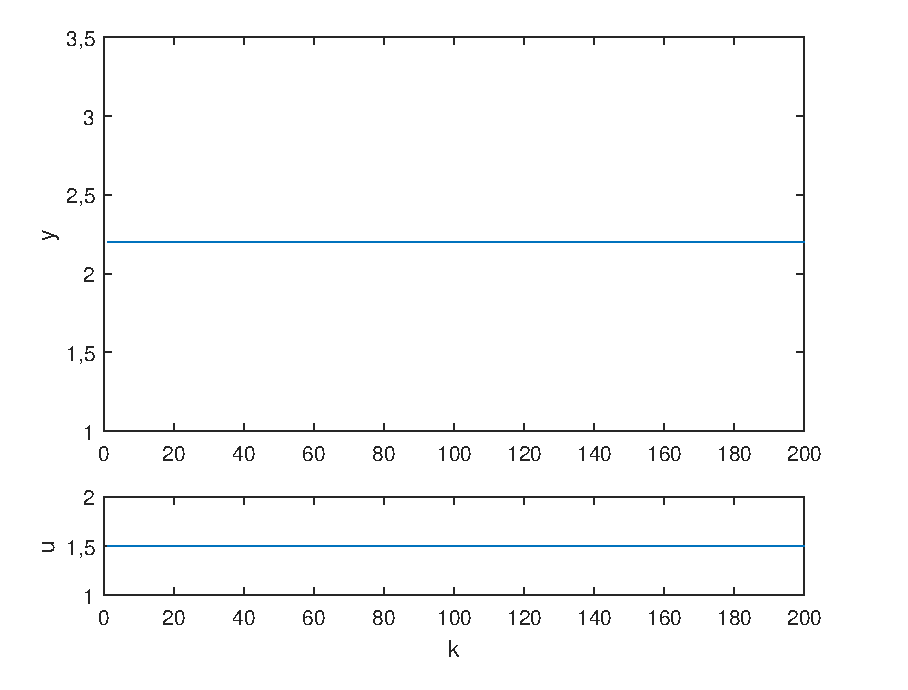
\includegraphics[scale=1]{images/Z1}
\caption{Odpowiedź procesu w punkcie pracy}
\label{Z1}
\end{figure}


\chapter{Podpunkt 2}
Po uwzględnieniu ograniczeń wartości sygnału sterującego dla reprezentacji odpowiedzi skokowych wybranych zostało sześć różnych wartości zmian sygnału sterującego: od $U_{pp}$ do $U_s$, w chwili $k=20$. Wykres odpowiedzi skokowych zamieszczony został na rys. \ref{Z2multiplesteps}.

\begin{figure}[ht]
\centering
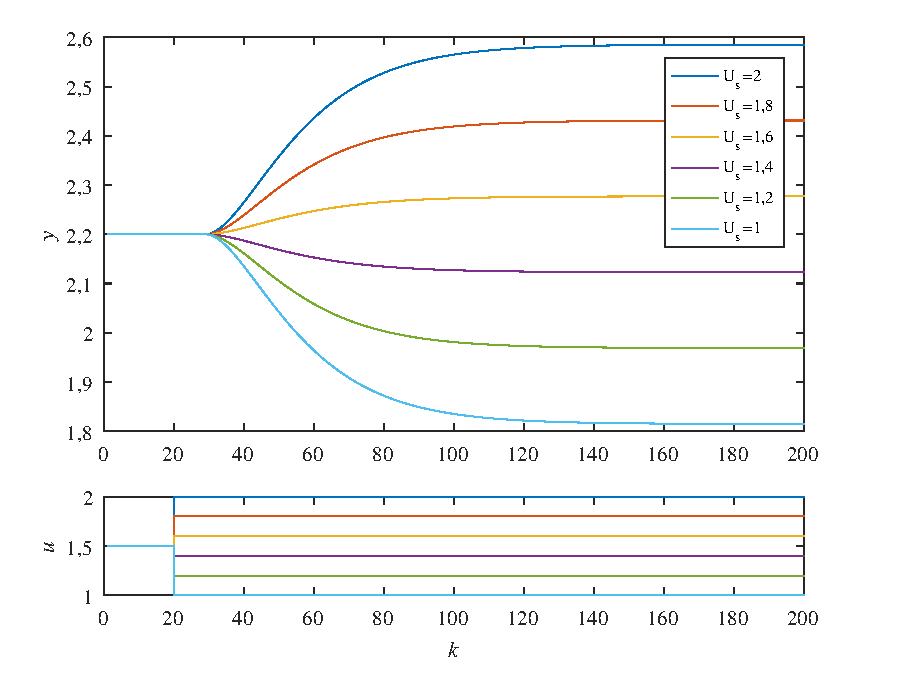
\includegraphics[scale=1]{images/Z2multiplesteps}
\caption{Wybrane odpowiedzi skokowe procesu}
\label{Z2multiplesteps}
\end{figure}

Symulując odpowiedź układu dla różnych wartości sygnału sterującego otrzymujemy charakterystykę statyczną $y(u)$ widoczną na rys. \ref{Z2staticchar}.


\begin{figure}[ht]
\centering
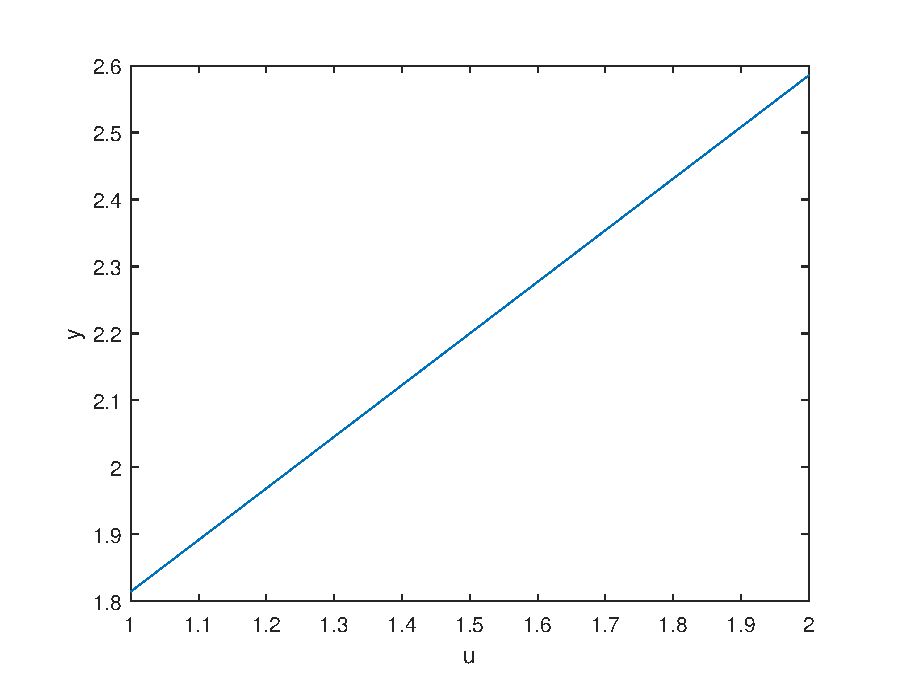
\includegraphics[scale=1]{images/Z2staticchar}
\caption{Charakterystyka statyczna procesu $y(u)$}
\label{Z2staticchar}
\end{figure}


Z odpowiedzi układu wnioskujemy, że zadany model jest samostabilizujący (statyczny), o opóźnieniu $\tau =10$, a jego charakterystyka statyczna jest w bardzo dobrym przybliżeniu liniowa. Obliczona wartość wzmocnienia statycznego procesu to $K=\num{0,7706}$.


\chapter{Podpunkt 3}
Na potrzeby algorytmu DMC przekształcona została odpowiedź skokowa dla skoku z punktu pracy o wartość dopuszczoną przez ograniczenia, t.j. dla skoku od $U_{\mathrm{pp}}=\num{1,5}$ do $U^{\mathrm{max}}=\num{2,0}$. Do przekształcenia wykorzystany został wzór (\ref{step_norm}), zaś uzyskana odpowiedź skokowa została przedstawiona na rys. \ref{Z3step}. Kolejne wartości wyznaczonej odpowiedzi skokowej zadanego modelu zapisane są w pliku \verb+step_responses.txt+.

\begin{equation}
S_i = \frac{S_i^0 - Y_{\mathrm{pp}}}{\triangle U} \textrm{, dla } i=1,\ldots
\label{step_norm}
\end{equation}


\begin{figure}[ht]
\centering
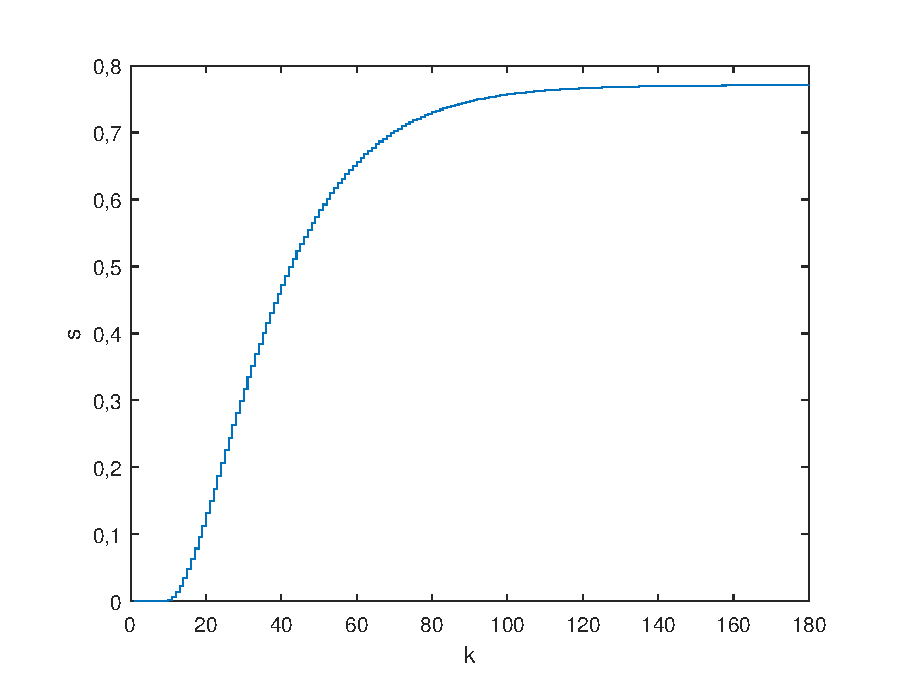
\includegraphics[scale=1]{images/Z3step}
\caption{Charakterystyka statyczna procesu $y(u)$}
\label{Z3step}
\end{figure}


\chapter{Podpunkt 4}
Programy do symulacji cyfrowej algorytmów PID oraz DMC (w wersji analitycznej) dla symulowanego procesu umieszczone zostały odpowiednio w plikach \verb+PID.m+, \verb+DMC.m+, zaś w plikach \verb+PID_err.m+ oraz \verb+DMC_err.m+ umieszczono funkcje pomocnicze do obliczania wartości błędu.

Symulacja cyfrowego algorytmu PID odbywa się w oparciu o postać dyskretną
\begin{equation}
r_2 = \frac{K T_{\mathrm{d}}}{T_{\mathrm{s}}} \
r_1 = K \left( \frac{T_{\mathrm{s}}}{2 T_{\mathrm{i}}} - \frac{2 T_{\mathrm{d}}}{T_{\mathrm{s}}} - 1 \right) \
r_0 = K \left( 1 + \frac{T_{\mathrm{s}}}{2 T_{\mathrm{i}}} + \frac{T_{\mathrm{d}}}{T_{\mathrm{s}}} \right) \\
\label{r_t}
\end{equation}
\begin{equation}
\triangle U(k) = r_2 e(k-2) + r_1 e(k-1) + r_0 e(k)
\label{du}
\end{equation}
gdzie $e(k)=Y^{\mathrm{zad}}(k) - Y(k)$ to uchyb. We wzorach (\ref{du2}--\ref{upp}) sterowanie jest przycinane zgodnie z ograniczeniami, a następnie przesuwane do punktu pracy.

\begin{equation}
\triangle U(k) = 
\begin{cases}
-\triangle U^{\mathrm{max}} &\quad \textrm{gdy } \ \triangle U(k) \le -\triangle U^{\mathrm{max}} \\
\triangle U^{\mathrm{max}} &\quad \textrm{gdy } \ \triangle U(k) \ge \triangle U^{\mathrm{max}}  \\
\triangle U(k) &\quad \textrm{w p.p.}
\end{cases}
\label{du2}
\end{equation}

\begin{equation}
U(k) = \triangle U(k) + U(k-1)
\label{uk}
\end{equation}

\begin{equation}
U(k) = 
\begin{cases}
U^{\mathrm{min}} - U_{\mathrm{pp}} &\quad \textrm{gdy } \ U(k) \le U^{\mathrm{min}}-U_{\mathrm{pp}} \\
U^{\mathrm{max}}-U_{\mathrm{pp}} &\quad \textrm{gdy } \ U(k) \ge U^{\mathrm{max}}-U_{\mathrm{pp}}  \\
U(k) &\quad \textrm{w p.p.}
\end{cases}
\label{uk2}
\end{equation}

\begin{equation}
U(k) = U(k) + U_{\mathrm{pp}}
\label{upp}
\end{equation}

Symulacja cyfrowa algorytmu DMC odbywa się w oparciu o wzory (\ref{YYdUk}--\ref{dukdmc}).

\begin{equation}
\boldsymbol{Y}^{\mathrm{zad}}(k)=\left[
\begin{array}{c}
y^{\mathrm{zad}}(k)\\
\vdots\\
y^{\mathrm{zad}}(k)
\end{array}
\right] \
\boldsymbol{U}(k)=\left[
\begin{array}{c}
y(k)\\
\vdots\\
y(k)
\end{array}
\right] \
\triangle \boldsymbol{U}(k)=\left[
\begin{array}{c}
\triangle u(k|k)\\
\vdots\\
\triangle u(k+N_{\mathrm{u}}-1|k)
\end{array}
\right] \
\label{YYdUk}
\end{equation}

\begin{equation}
\triangle \boldsymbol{U}^{\mathrm{P}}(k)=\left[
\begin{array}{c}
\triangle u(k-1)\\
\vdots\\
\triangle u(k-(D-1))
\end{array}
\right]
\label{dUp}
\end{equation}

\begin{equation}
\boldsymbol{M}=\left[
\begin{array}
{cccc}
s_{1} & 0 & \ldots & 0\\
s_{2} & s_{1} & \ldots & 0\\
\vdots & \vdots & \ddots & \vdots\\
s_{N} & s_{N-1} & \ldots &  s_{N-N_{\mathrm{u}}+1}
\end{array}
\right]
\label{Marray}
\end{equation}

\begin{equation}
\boldsymbol{M}^{\mathrm{P}}=\left[
\begin{array}
{cccc}
s_{2} - s_{1} & s_{3} - s_{2} & \ldots & s_{\mathrm{D}} - s_{\mathrm{D-1}}\\
s_{3} - s_{1} & s_{4} - s_{2} & \ldots & s_{\mathrm{D+1}} - s_{\mathrm{D-1}}\\
\vdots & \vdots & \ddots & \vdots\\
s_{N+1} - s_{1} & s_{N+2} - s_{2} & \ldots & s_{\mathrm{N+D-1}} - s_{\mathrm{D-1}}\\
\end{array}
\right]
\label{MParray}
\end{equation}

\begin{equation}
\boldsymbol{Y}^{0}(k) = \boldsymbol{Y}(k) + \boldsymbol{M}^{\mathrm{P}} \triangle \boldsymbol{U}^{\mathrm{P}}(k)
\label{Y0k}
\end{equation}

\begin{equation}
\boldsymbol{K} = (\boldsymbol{M}^{\mathrm{T}} \boldsymbol{M} + \lambda \boldsymbol{I})^{-1} \boldsymbol{M}^{\mathrm{T}}
\label{Karray}
\end{equation}

\begin{equation}
\triangle \boldsymbol{U}(k) = \boldsymbol{K}(\boldsymbol{Y}^{\mathrm{zad}}(k) - \boldsymbol{Y}^{0}(k))
\label{dukdmc}
\end{equation}

Ponieważ w zadanym przypadku do regulacji wykorzystywane są jedynie sygnały z chwili $k$ liczenie ich w dalszych chwilach może być w tym przypadku pominięte. Dla przyspieszenia działania symulacji używany jest więc tylko pierwszy wiersz macierzy $\boldsymbol{K}$ oznaczony tutaj przez $\boldsymbol{K}_1$ - za jego pomocą liczona jest wartość sterowania jedynie w chwili aktualnej:

\begin{equation}
	\triangle u(k|k) = \boldsymbol{K}_1 (\boldsymbol{Y}^{\mathrm{zad}}(k) - \boldsymbol{Y}^{0}(k))
\end{equation}

\chapter{Podpunkt 5}
Wybrane przez nas regulatory oceniano jakościowo na podstawie przebiegów - preferowane były przebiegi odpowiednio gładkie, bez wyraźnych oscylacji oraz z niewielkim, bądź niewystępującym przeregulowaniem, które były bliskie do zadanego przebiegu - oraz ilościowo, zgodnie z zadanym wskaźnikiem jakości regulacji
\begin{equation}
E = \sum_{k=1}^{k_{\mathrm{konc}}}(y^{\mathrm{zad}}(k) - y(k))^2
\label{E}
\end{equation}
gdzie za koniec symulacji przyjęto $k_{\mathrm{konc}}=3000$. Wartości wyjść zadane w symulacji przedstawiono na poniższych wykresach za pomocą pomarańczowej, przerywanej linii.

\begin{figure}[ht]
\centering
\makebox[\textwidth][c]{
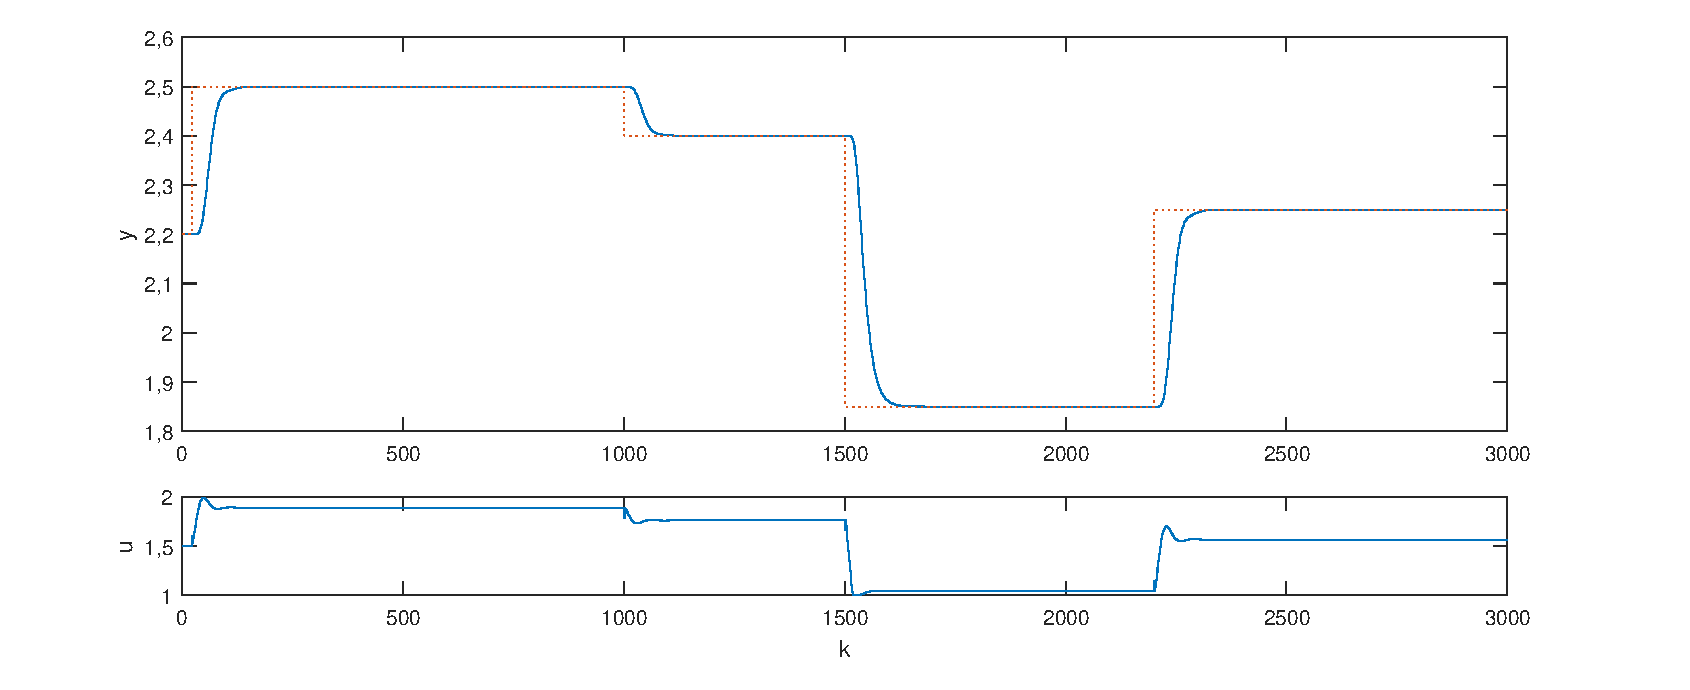
\includegraphics[scale=1]{images/Z5manualPID}}
\caption{Wyniki symulacji dla dobranego eksperymentalnie regulatora PID: \\$K = \num{2,64}$, $T_{\mathrm{i}}=\num{14,00}$, $T_{\mathrm{d}}=\num{3,36}$, wyznaczony błąd $E=\num{19,6632}$}
\label{Z5manualPID}
\end{figure}


\begin{figure}[ht]
\centering
\makebox[\textwidth][c]{
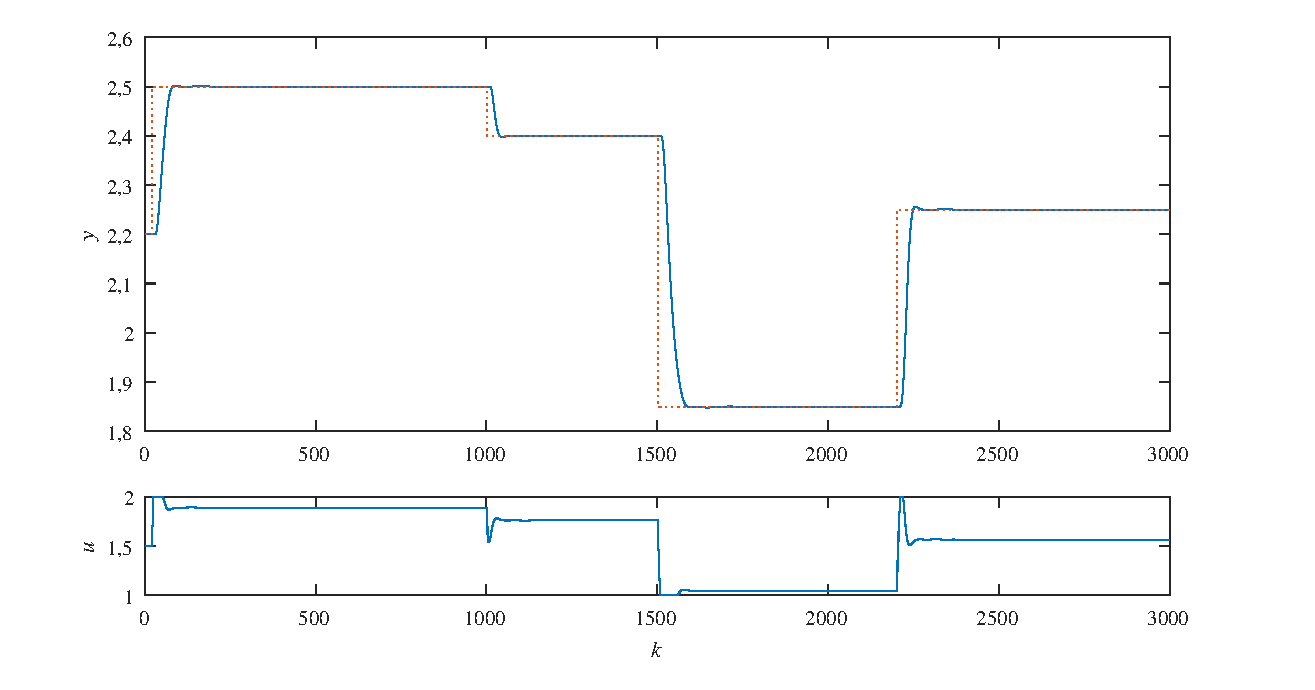
\includegraphics[scale=1]{images/Z5manualDMC}}
\caption{Wyniki symulacji dla dobranego eksperymentalnie regulatora DMC: \\$N=30$, $N_{\mathrm{u}}=3$, $\lambda=\num{0,8}$, wyznaczony błąd $E=\num{15,6111}$}
\label{Z5manualDMC}
\end{figure}

\chapter{Podpunkt 6}
Optymalizacja wskaźnika jakości została przeprowadzona przy użyciu skryptu zamieszczonego w pliku \verb+param_optimizer.m+, do optymalizacji globalnej wykorzystuje on funkcję \verb+ga+(algorytm genetyczny). Przy jego użyciu zmodyfikowane jednak zostały zadane wartości wyjściowe - wydłużono czasy między skokami. Bez zrobienia tego, przy symulacji regulatora z otrzymanymi parametrami układ wpadał w znaczące oscylacje - priorytetyzowane okazywało się wtedy jak najszybsze przejście do nowej wartości ze skoku ponad wygładzenie sygnału ustalonego. Wydłużenie czasów pomaga tego uniknąć, choć niejakie oscylacje nadal są widoczne w zoptymalizowanym regulatorze PID.

Przy optymalizacji algorytmem genetycznym dla obu regulatorów użyto losowych populacji (parametrów) początkowych. Program uruchomiono kilkukrotnie, uzyskując za każdym razem bardzo zbliżone wyniki. 

Ograniczenia nałożone na przeszukiwane wartości dla regulatora PID to:
\begin{equation}
	0.01 \le K, \quad
	1 \le T_\mathrm{i},\quad
	0.01 \le T_\mathrm{d}
\end{equation}

a dla regulatora DMC przy parametrze $D=120$:
\begin{equation}
	1 \le N_\mathrm{u} \le N \le 180, \quad 
	0.01 \le \lambda
\end{equation}


Dla przejrzystości wykresów zoptymalizowanych regulatorów przedstawiono na nich symulację przy przebiegu czasowym wartości zadanych wziętym z poprzedniego zadania, bez wydłużenia okresów między kolejnymi skokami.

\begin{figure}[ht]
\centering
\makebox[\textwidth][c]{
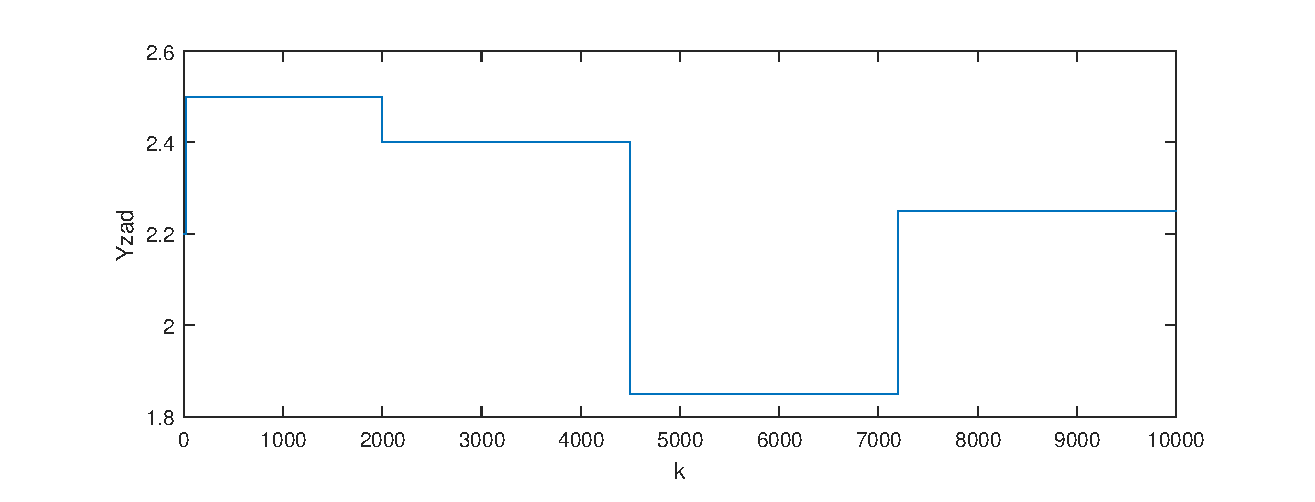
\includegraphics[scale=1]{images/Z6Yzad}}
\caption{Przebieg czasowy wartości zadanych dla regulatorów użyty przy optymalizacji wskaźnika jakości}
\label{Z6optimizedPID}
\end{figure}

\begin{figure}[ht]
\centering
\makebox[\textwidth][c]{
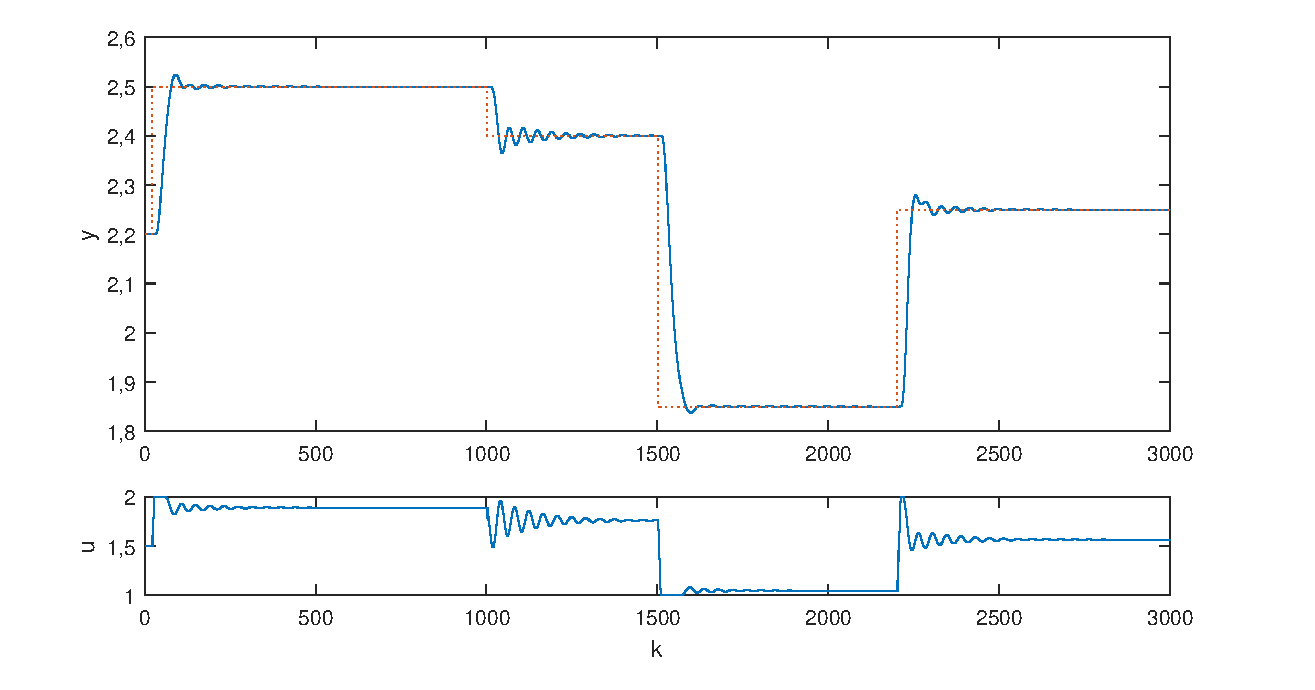
\includegraphics[scale=1]{images/Z6optimizedPID}}
\caption{Wyniki symulacji dla regulatora PID otrzymanego w wyniku optymalizacji:\\ $K=\num{5,422910}$, $T_{\mathrm{i}}=\num{8,551461}$, $T_{\mathrm{d}}=\num{3,914535}$, wyznaczony błąd $E=\num{16,7418}$}
\label{Z6optimizedPID}
\end{figure}

\begin{figure}[ht]
\centering
\makebox[\textwidth][c]{
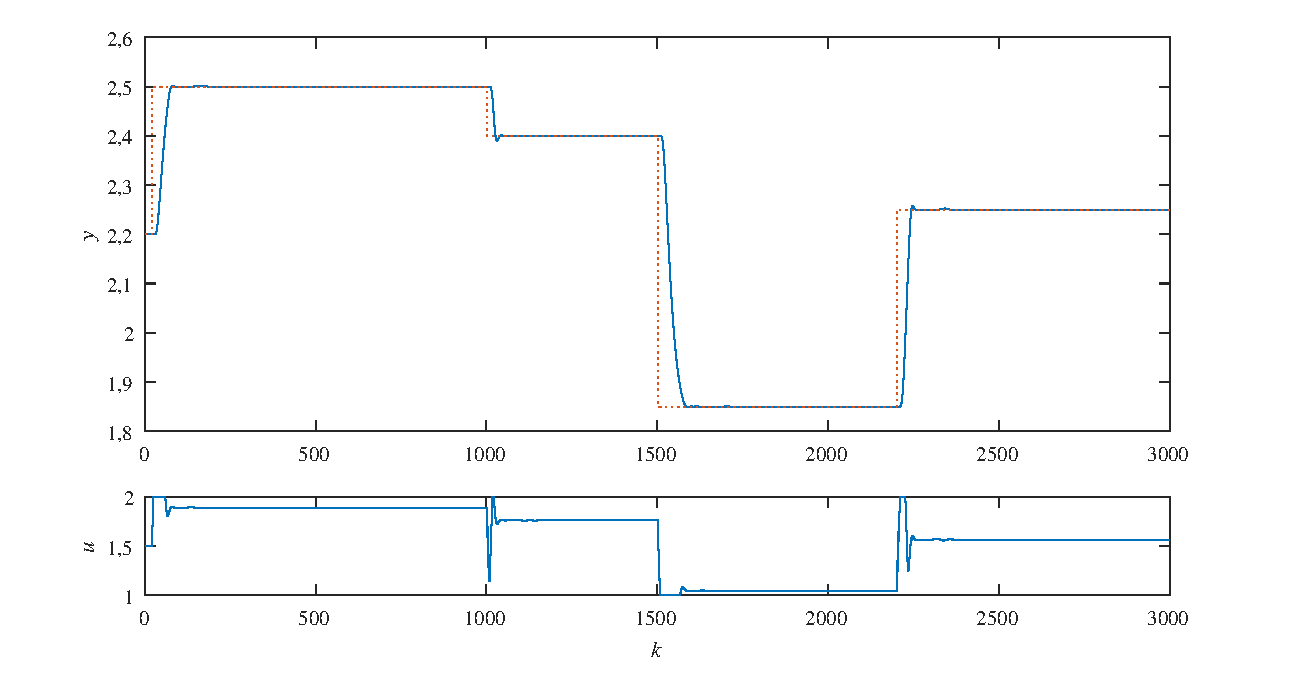
\includegraphics[scale=1]{images/Z6optimizedDMC.eps}}
\caption{Wyniki symulacji dla regulatora DMC otrzymanego w wyniku optymalizacji:\\ $N=33$, $N_{\mathrm{u}}=4$, $\lambda=\num{0,018527}$, wyznaczony błąd $E=\num{15,5746}$}
\label{Z6optimizedDMC}
\end{figure}
